\begin{frame}
\frametitle{Continued fractions}

Representing $\alpha$ as a continued fraction:
\begin{equation*}
	\alpha =
	[a_0; a_1, a_2, ...] =
	a_0 + \dfrac{1}{\normalsize a_1 + \dfrac{1}{a_2 + \dfrac{1}{\ddots}}},\;\;
	a_0 \in \mathbb{Z},\; a_1, a_2, ... \in \mathbb{N}.
\end{equation*}

The continued fraction produces infinitely many rational convergents of $\alpha$:
\begin{equation*}
	\alpha_n = \dfrac{P_n}{Q_n} = [a_0; a_1, a_2, ..., a_n].
\end{equation*}

The sequence $\{\alpha_n\}$ converges to $\alpha$:
\begin{figure}[c]
	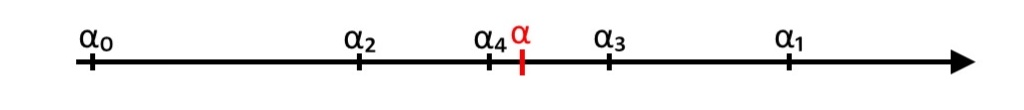
\includegraphics[width=0.8\textwidth]{convergents}
\end{figure}

\end{frame}
